\section{General Modeling Overview}\label{general-modeling-overview}

The EnergyPlus program is a collection of many program modules that work together to calculate the energy required for heating and cooling a building using a variety of systems and energy sources. It does this by simulating the building and associated energy systems when they are exposed to different environmental and operating conditions. The core of the simulation is a model of the building that is based on fundamental heat balance principles. Since it is relatively meaningless to state: ``based on fundamental heat balance principles'', the model will be described in greater detail in later sections of this document in concert with the C++ code which is used to describe the model. It turns out that the model itself is relatively simple compared with the data organization and control that is needed to simulate the great many combinations of system types, primary energy plant arrangements, schedules, and environments. Figure \ref{fig:energyplus-program-schematic} shows this overall organization in schematic form. Later sections will expand on the details within the blocks of the schematic.

\begin{figure}[hbtp] % fig 1
\centering
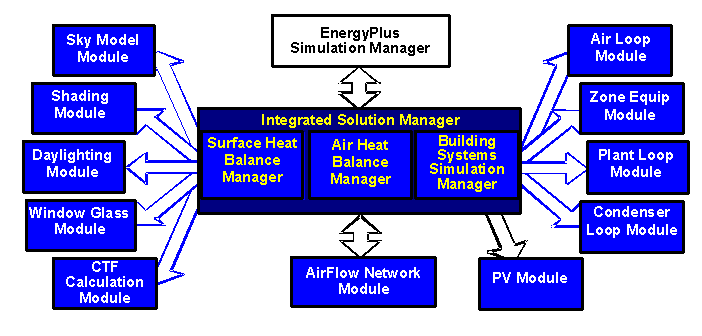
\includegraphics[width=0.9\textwidth, height=0.9\textheight, keepaspectratio=true]{media/image1.png}
\caption{EnergyPlus Program Schematic \protect \label{fig:energyplus-program-schematic}}
\end{figure}

\section{Building Surfaces, Spaces, Zones, and Enclosures}\label{building-spaces-zones-enclosures}
The EnergyPlus building model consists of four main constructs: surfaces, spaces, zones, and enclosures. These are defined below along with some assumptions and relationship rules.

\begin{description}
  \item[Surface] - a geometric plane which is attached to a Zone and a Space.
  \begin{itemize}
    \item
     A Surface can be opaque, transparent, or an air boundary.
    \item
     Surfaces may store and transfer heat and moisture.
    \item
     The inside and outside face of each Surface has a single uniform surface temperature calculated from the surface heat balance.
    \item
     Each Surface belongs to one Zone and one Space.
    \item
     Inter-Space and inter-Zone Surfaces are modeled as two linked surfaces.
    \item
     Air boundary surfaces combine one or more spaces into a common enclosure.
    \item
     Inter-Space surfaces connecting spaces that are part of the same Zone will see the same air temperature. They may or may not be in the same enclosure.
    \item
     Inter-Space surfaces connecting spaces that are in different Zones may see different air temperatures. They may or may not be in the same enclosure.
  \end{itemize}

  \item[Space] - A collection of one or more Surfaces and internal gains.
  \begin{itemize}
    \item
     Each Space belongs to one Zone.
    \item
     Spaces may be user-specified or generated by default so that every surface belongs to a Space and every Zone has at least one Space.
    \item
     A Space may have only floor surface(s) or may be fully enclosed (floors, walls, ceilings, etc).
    \item
     Each Space belongs to one Enclosure (implicitly assigned). See Enclosure below for more details.
    \item
     There is no heat balance at the Space level; the heat balance is done at the Zone level.
    \item
     Internal gains are modeled at the Space level and combined for the Zone heat balance.
    \item
     Each Space is assigned a Space Type which is used for output reports and submeters.
  \end{itemize}

  \item[Zone] - An air mass connecting Surfaces, internal gains, and HVAC equipment for heat balance and HVAC control.
  \begin{itemize}
    \item
     Each Zone is comprised of one or more Spaces.
    \item
     If no Spaces are specified for a Zone, a Space will automatically be created.
    \item
     If any surfaces in a Zone do not have a user-assigned Space, a Space will be automatically created for those surfaces.
    \item
     The Zone heat balance solves for the zone air temperature and humidity (or a Room Air Model with multiple air nodes) and includes all Surfaces and internal gains from its Spaces. 
    \item
     HVAC systems are connected at the Zone level.
  \end{itemize}

  \item[Enclosure] - A continuous volume connecting Surfaces for radiant, solar, and daylighting exchange.
  \begin{itemize}
    \item
     Each Enclosure is comprised of one or more Spaces.
    \item
     If a Space has a floor surface(s) plus any other surfaces (walls, ceiling, roof, etc.), then it is its own enclosure.
    \item
     If a Space has only a floor surface(s), then it is part of the zone enclosure.
    \item
     Any surfaces with a blank Space is part of the zone enclosure.
    \item
     Air boundaries can be used to combine Spaces into a common enclosure.
    \item
     All Surfaces and internal radiant gains associated with the Spaces are included in the Enclosure.
    \item
     Enclosures only distribute radiant (thermal), solar, and visible energy to and from the Surfaces.
    \item
     There is no full heat balance at the Enclosure level. Each Enclosure only balances the radiant/solar flux on each Surface. These fluxes then become part of the Surface inside heat balance.
  \end{itemize}
\end{description}
